%%%% COMPARISON TO THIERGART'S METHOD %%%%
\chapter{Comparison to time-frequency analysis and sound field modeling}\label{chap:09_Thiergart_Comparison}
In this chapter, we present a comparison of the time-frequency navigational method of \citet{Thiergart2013}, described here in 
\secref{sec:03_Navigation_Techniques:Thiergart_Method}, and our parametric method proposed in \chapref{chap:08_Proposed_Method}.
To that end, we present a characterization of the time-frequency method via numerical simulations that are nearly identical to those presented in \secref{sec:08_Proposed_Method:Results}.
Through these analyses, we aim to derive practically-relevant principles that will inform decisions regarding which method to use under various conditions or for different applications.

%% saved for a paper abstract
%Results of these simulations show that each method offers advantages in different regimes of parameters (e.g., microphone spacing, source distance, etc.), and consequently the choice of method should be determined based on its intended application.
%For example, the time-frequency method may be preferable for large-area recordings and when spatial localization accuracy is critical, as this method yields superior localization performance (compared to the proposed method) at large microphone spacings ($>1$~m).
%However, the proposed method may be more suitable for many consumer applications in which sound quality attributes such as coloration and diffuseness are more important, since this method achieves smaller spectral errors at large microphone spacings and smaller diffuseness errors under all conditions.

\section{Simulations}\label{sec:09_Thiergart_Comparison:Simulations}
We conduct simulations of the time-frequency interpolation method following the simulation framework laid out in \chapref{chap:06_Simulation_Framework}.
However, note that for this method, we intentionally omit source azimuths of $\varphi_0 = 90^\circ$.
This is necessary since, for a source azimuth of $\pm90^\circ$, the source becomes collinear with the microphones and consequently the triangulation calculation (see \eqnref{eq:03_Navigation_Techniques:Source_Triangulation}) can no longer produce a unique solution.
Also, recall that the time-frequency method has only been derived for first-order ambisonics input signals (see \secref{sec:03_Navigation_Techniques:Thiergart_Method}), so we must choose $L_\text{in} = 1$ for this method.

For ease of comparison, we also reproduce in this chapter the simulation results presented in \chapref{chap:08_Proposed_Method} for our proposed parametric interpolation method.
Note, however, that in those simulations we included source azimuths of $\varphi_0 = 90^\circ$ and chose $L_\text{in} = 4$.
(Recall from \secref{sec:08_Proposed_Method:Order_Dependence} that the performance of our proposed method does not vary significantly with order.)

\section{Source azimuth dependence}\label{sec:09_Thiergart_Comparison:Azimuth_Dependence}
In this section, we examine the effective frequency response induced by translation via the time-frequency interpolation method as a function of source azimuth.
As described in \secref{sec:06_Simulation_Framework:Azimuth_Dependence}, for these simulations, we pick $\Delta = 0.5$~m and $s_0 = 2.5$~m (so $\gamma = 10$), and interpolate to $\vec{r}_0 = (0, 0, 0)$.
(Recall that these quantities are defined in \secref{sec:06_Simulation_Framework:Linear_Geometry} for a linear array geometry.)

The induced frequency responses are plotted in \figref{fig:09_Thiergart_Comparison:Azimuth_Dependence} for both the time-frequency interpolation method and our proposed parametric interpolation method (see \chapref{chap:08_Proposed_Method}).
From \figref{fig:09_Thiergart_Comparison:Azimuth_Dependence:Thiergart}, we see that the time-frequency interpolation method tends to produce a comb-filtering response, similar to that of the weighted average method (see \figref{fig:08_Proposed_Method:XF_CombFiltering}), but with much shallower notches.

\begin{figure*}[t]
  \centering
  \begin{subfigure}[b]{0.49\textwidth}
    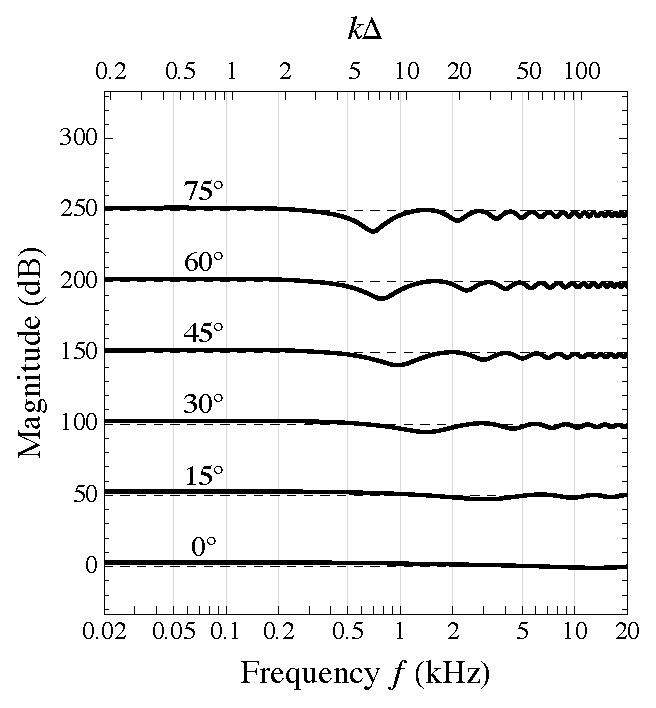
\includegraphics[width=\textwidth]{09_thiergart_comparison/figures/sourceAz_freqResp_thiergart.eps}
    \caption{\citet{Thiergart2013} method}
    \label{fig:09_Thiergart_Comparison:Azimuth_Dependence:Thiergart}
  \end{subfigure}
  \hfill
  \begin{subfigure}[b]{0.49\textwidth}
    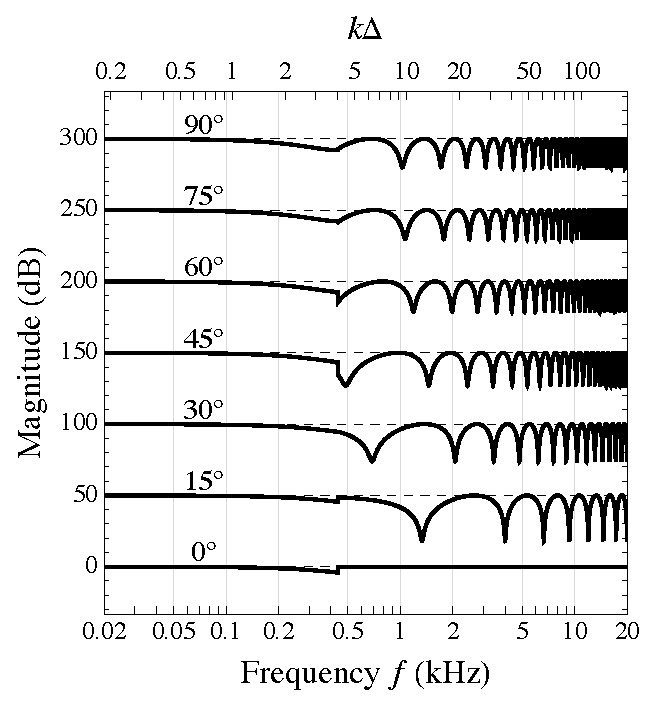
\includegraphics[width=\textwidth]{08_proposed_method/figures/sourceAz_freqResp_validhybrid.eps}
    \caption{Proposed method}
    \label{fig:09_Thiergart_Comparison:Azimuth_Dependence:Hybrid}
  \end{subfigure}

  \caption[Magnitude responses across azimuths for each interpolation method.]{
  Magnitude responses caused by the time-frequency and proposed interpolation methods for various source azimuths.
  The bottom axes show frequency in kHz while the top axes show the nondimensional frequency $k\Delta$ for a microphone spacing of $\Delta = 0.5$~m.
  For legibility, each frequency response is offset by $50$~dB and the responses have been artificially truncated (where needed) to not exceed $-45$~dB.
  \Figref{fig:09_Thiergart_Comparison:Azimuth_Dependence:Hybrid} has been reproduced from \figref{fig:08_Proposed_Method:Azimuth_Dependence:Hybrid}.}
  \label{fig:09_Thiergart_Comparison:Azimuth_Dependence}
\end{figure*} %%NOTE%% vertical axis label is too complicated: |A0 / B0ref| or something

These notches also tend to be wider and spaced farther apart than those of the the comb-filtering response.
Consequently, they may in fact lead to comparably-perceptible coloration, as it is well-established that wider notches are more audible than narrow ones \citep{Bucklein1981}.
Correspondingly, in terms of the computed spectral error (see \eqnref{eq:ABSE}), a wide but shallow notch may yield a comparable spectral error as does a narrow but deep notch once averaged over frequency (due to the effective spectral ``smoothing'' that results from the bank of gammatone filters).

As discussed in \secref{sec:08_Proposed_Method:Azimuth_Dependence}, the frequency response induced by translation via the proposed method (shown in \figref{fig:09_Thiergart_Comparison:Azimuth_Dependence:Hybrid}) consists of a largely flat response at low frequencies concatenated with a comb-filter response at high frequencies.
Psychoacoustic studies have shown that comb-filter responses can be imperceptible if the time-delay between the primary and secondary signals is long enough and/or if their relative levels are different enough \citep{Kates1984,Brunner2007}.
As a result, even though the comb-filter notches shown in \figref{fig:09_Thiergart_Comparison:Azimuth_Dependence:Hybrid} are significantly deeper than those shown in \figref{fig:09_Thiergart_Comparison:Azimuth_Dependence:Thiergart}, it is not necessarily the case that the former will yield more audible coloration than the latter.
This issue will be explored specifically in the following section.
%Ultimately, subjective listening tests may be needed to definitively establish the audibility of the particular colorations induced by each method.

%It should be emphasized that the above plots only illustrate a single condition ($\Delta = 0.5$~m, $\gamma = 10$, and $\vec{r}_0 = (0,0,0)$), so a more comprehensive exploration is required, as will be presented in the following section.

\section{Characterization and discussion}\label{sec:09_Thiergart_Comparison:Results}
As mentioned above, the triangulation step of the time-frequency method fails for source azimuths of $|\varphi_0| = 90^\circ$.
Consequently, for this method only, we have varied the source azimuth only from $\varphi_0 = 0^\circ$ to $85^\circ$ in increments of $5^\circ$ and averaged over these azimuths.

% Level

In \figref{fig:09_Thiergart_Comparison:Level_Errors:Thiergart}, we plot the level errors (as defined in \secref{sec:04_Auditory_Models:Audible_Energy}) incurred by the time-frequency method as a function of array spacing $\Delta$ and normalized source distance $\gamma$.
For ease of comparison with the proposed navigational method, in this section we have reproduced the corresponding contour plots (e.g., \figref{fig:09_Thiergart_Comparison:Level_Errors:Hybrid}) from \secref{sec:08_Proposed_Method:Results}.
From \figref{fig:09_Thiergart_Comparison:Level_Errors:Thiergart}, we see that the time-frequency method is able to achieve approximately zero error almost everywhere, with the exception of far interior sources ($\gamma < 1$).
This yields an improvement over the proposed method, which is only able to accurately reconstruct the sound level for exterior sources ($\gamma > 1$) and is otherwise several dB too quiet for interior sources.

\begin{figure*}[t]
	\centering
	\begin{subfigure}[b]{0.49\textwidth}
		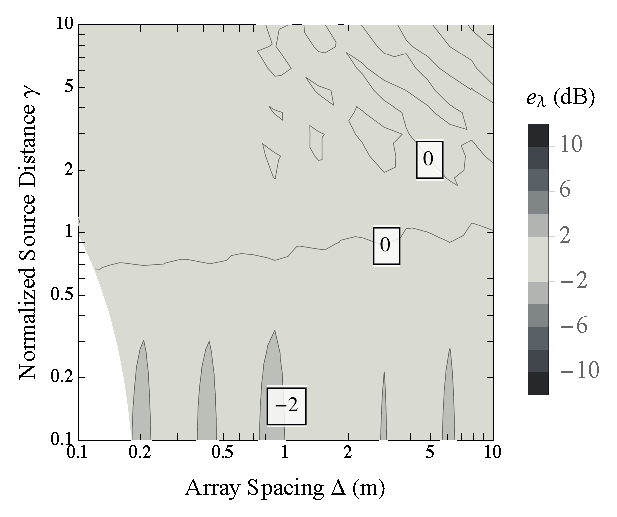
\includegraphics[width=\textwidth]{09_thiergart_comparison/figures/audibleEnergy_contour_thiergart.eps}
		\caption{\citet{Thiergart2013} method}
		\label{fig:09_Thiergart_Comparison:Level_Errors:Thiergart}
	\end{subfigure}
	\hfill
	\begin{subfigure}[b]{0.49\textwidth}
		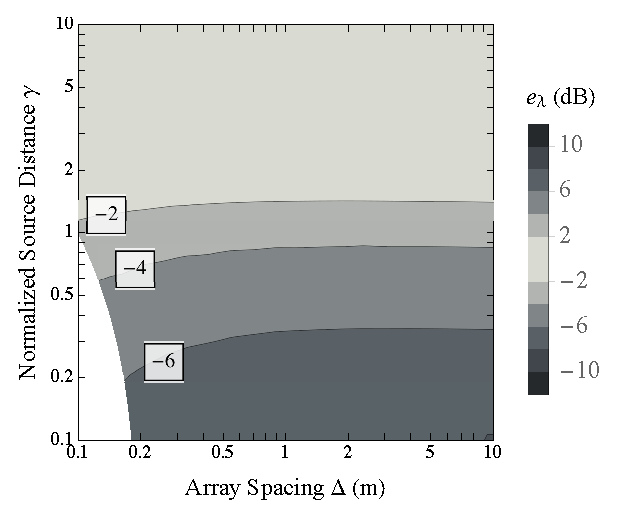
\includegraphics[width=\textwidth]{08_proposed_method/figures/audibleEnergy_contour_validhybrid.eps}
		\caption{Proposed method}
		\label{fig:09_Thiergart_Comparison:Level_Errors:Hybrid}
	\end{subfigure}
	
	\caption[Contour plots of level errors for each interpolation method.]{
	Level errors $e_\lambda$ for microphone spacing $\Delta$ and normalized source distance $\gamma$.
  Contour lines are drawn every $2$~dB.
  \Figref{fig:09_Thiergart_Comparison:Level_Errors:Hybrid} has been reproduced from \figref{fig:08_Proposed_Method:Level_Errors:Hybrid}.}
	\label{fig:09_Thiergart_Comparison:Level_Errors}
\end{figure*}

% Coloration

For spectral coloration, however, we see in \figref{fig:09_Thiergart_Comparison:Spectral_Errors:Thiergart} that the time-frequency method yields larger spectral errors (as defined in \secref{sec:04_Auditory_Models:Coloration_Metrics:ABSE}) than the proposed method for all microphone spacings larger than approximately $0.5$~m.
In particular, the proposed method yields significantly smaller errors for interior sources with large microphone spacings ($\gamma < 1$ and $\Delta > 0.5$~m).
Only for exterior sources with microphone spacings smaller than approximately $0.25$~m does the time-frequency method achieve smaller spectral errors than the proposed method.
As the precise origin of the spectral coloration induced by translation via the time-frequency method remains unclear, future investigations should attempt to determine the source of, and ideally correct for, such colorations.

\begin{figure*}[t]
	\centering
	\begin{subfigure}[b]{0.49\textwidth}
		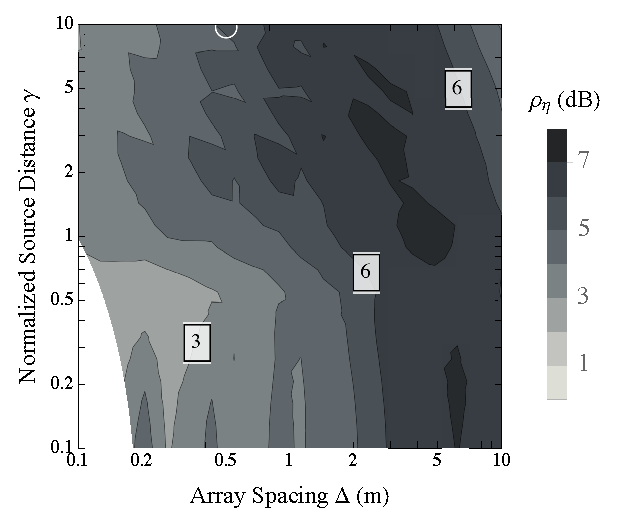
\includegraphics[width=\textwidth]{09_thiergart_comparison/figures/scharer2009_contour_thiergart_marked.eps}
		\caption{\citet{Thiergart2013} method}
		\label{fig:09_Thiergart_Comparison:Spectral_Errors:Thiergart}
	\end{subfigure}
	\hfill
	\begin{subfigure}[b]{0.49\textwidth}
		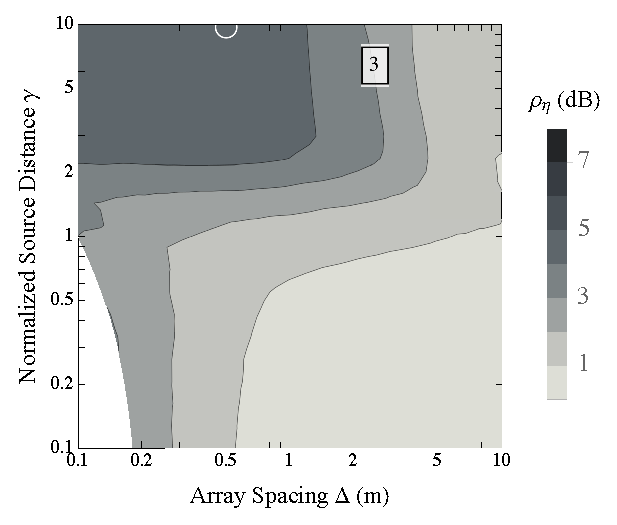
\includegraphics[width=\textwidth]{09_thiergart_comparison/figures/scharer2009_contour_validhybrid_marked.eps}
		\caption{Proposed method}
		\label{fig:09_Thiergart_Comparison:Spectral_Errors:Hybrid}
	\end{subfigure}
	
	\caption[Contour plots of spectral errors for each interpolation method.]{
	Spectral errors $\rho_\eta$ for microphone spacing $\Delta$ and normalized source distance $\gamma$.
  Contour lines are drawn every $1$~dB.
  The white semicircles indicate the conditions shown in \figref{fig:09_Thiergart_Comparison:Azimuth_Dependence}, where $\Delta = 0.5$~m and $\gamma = 10$.
  \Figref{fig:09_Thiergart_Comparison:Spectral_Errors:Hybrid} has been reproduced from \figref{fig:08_Proposed_Method:Spectral_Errors:Hybrid}.}
	\label{fig:09_Thiergart_Comparison:Spectral_Errors}
\end{figure*}

Recalling the discussion in \secref{sec:09_Thiergart_Comparison:Azimuth_Dependence}, we now see that the spectral errors corresponding to the conditions shown in \figref{fig:09_Thiergart_Comparison:Azimuth_Dependence} (with $\Delta = 0.5$~m and $\gamma = 10$) are indeed comparable:
at that point in \figreftwo{fig:09_Thiergart_Comparison:Spectral_Errors:Thiergart}{fig:09_Thiergart_Comparison:Spectral_Errors:Hybrid}, the time-frequency method yields a spectral error of approximately 5~dB and the proposed method yields a spectral error between 4 and 5~dB.
To understand this apparent discrepancy between \figreftwo{fig:09_Thiergart_Comparison:Azimuth_Dependence}{fig:09_Thiergart_Comparison:Spectral_Errors}, it should be recalled that the spectral error calculation effectively ``smooths'' the frequency responses via averaging over a bank of gammatone filters (see \eqnref{eq:ABSE}).
It should also be emphasized that the frequency response plots shown in \figref{fig:09_Thiergart_Comparison:Azimuth_Dependence} only illustrate a single condition ($\Delta = 0.5$~m, $\gamma = 10$, and $\vec{r}_0 = (0,0,0)$), whereas the data shown in \figref{fig:09_Thiergart_Comparison:Spectral_Errors} have been averaged over the entire navigable region and all source azimuths.

% Localization

Localization errors (as computed with \eqnref{eq:04_Auditory_Models:Localization_Error} for the localization model described in \secref{sec:05_Proposed_Models:Localization_Model}) for the time-frequency method are shown in \figref{fig:09_Thiergart_Comparison:Localization_Errors:Thiergart}.
Contrary to that method's coloration performance (see \figref{fig:09_Thiergart_Comparison:Spectral_Errors:Thiergart}), which is most accurate at small microphone spacings (e.g., $\Delta < 0.5$~m), the localization errors incurred by this method are largest at those small microphone spacings.
In particular, for exterior sources with microphone spacings smaller than approximately $0.3$~m, the proposed method yields a significant improvement ($\sim15^\circ$) over the time-frequency method.
Additionally, for far exterior sources ($\gamma > 3$) and at all microphone spacings, the proposed method yields a reasonably large improvement ($\sim5^\circ$) over the time-frequency method.
For microphone spacings larger than approximately $0.5$~m, the errors incurred by the proposed method are relatively constant with spacing, whereas those incurred by the time-frequency method improve with increasing spacing and even become very small ($\epsilon_\nu < 5^\circ$) at large $\Delta$ and $\gamma < 1$.
Accordingly, the time-frequency method yields a significant improvement over the proposed method for interior sources with microphone spacings larger than approximately $1$~m.

\begin{figure*}[t]
	\centering
	\begin{subfigure}[b]{0.49\textwidth}
		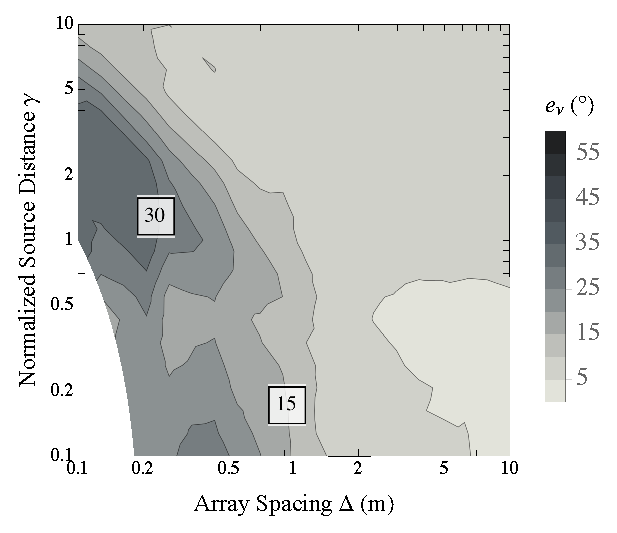
\includegraphics[width=\textwidth]{09_thiergart_comparison/figures/tylka2017_contour_thiergart.eps}
		\caption{\citet{Thiergart2013} method}
		\label{fig:09_Thiergart_Comparison:Localization_Errors:Thiergart}
	\end{subfigure}
	\hfill
	\begin{subfigure}[b]{0.49\textwidth}
		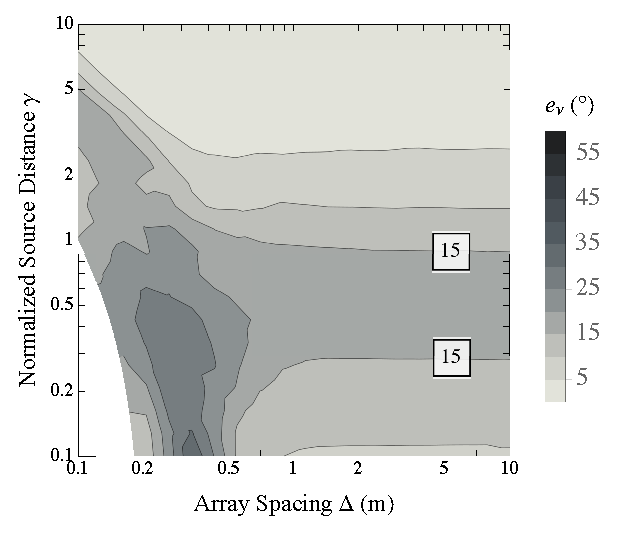
\includegraphics[width=\textwidth]{08_proposed_method/figures/tylka2017_contour_validhybrid.eps}
		\caption{Proposed method}
		\label{fig:09_Thiergart_Comparison:Localization_Errors:Hybrid}
	\end{subfigure}
	
	\caption[Contour plots of localization errors for each interpolation method.]{
	Predicted localization errors $e_\nu$ for microphone spacing $\Delta$ and normalized source distance $\gamma$.
	Contour lines are drawn every $5^\circ$.
	\Figref{fig:09_Thiergart_Comparison:Localization_Errors:Hybrid} has been reproduced from \figref{fig:08_Proposed_Method:Localization_Errors:Hybrid}.}
	\label{fig:09_Thiergart_Comparison:Localization_Errors}
\end{figure*}

% Diffuseness

From the plots of diffuseness errors (see \secref{sec:04_Auditory_Models:Diffuseness_Parameter}) shown in \figreftwo{fig:09_Thiergart_Comparison:Diffuseness_Errors:Thiergart}{fig:09_Thiergart_Comparison:Diffuseness_Errors:Hybrid}, we immediately see that the proposed method achieves more accurate performance than the time-frequency method over all conditions.
The time-frequency method consistently yields a diffuseness parameter which is too small, whereas the proposed method achieves nearly exact diffuseness (except at very small $\gamma$ and $\Delta$).

\begin{figure*}[t]
	\centering
	\begin{subfigure}[b]{0.49\textwidth}
		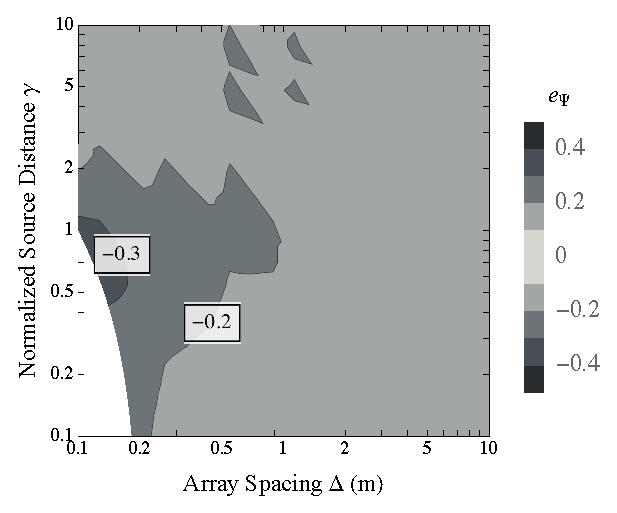
\includegraphics[width=\textwidth]{09_thiergart_comparison/figures/merimaa2005_d_contour_thiergart.eps}
		\caption{\citet{Thiergart2013} method}
		\label{fig:09_Thiergart_Comparison:Diffuseness_Errors:Thiergart}
	\end{subfigure}
	\hfill
	\begin{subfigure}[b]{0.49\textwidth}
		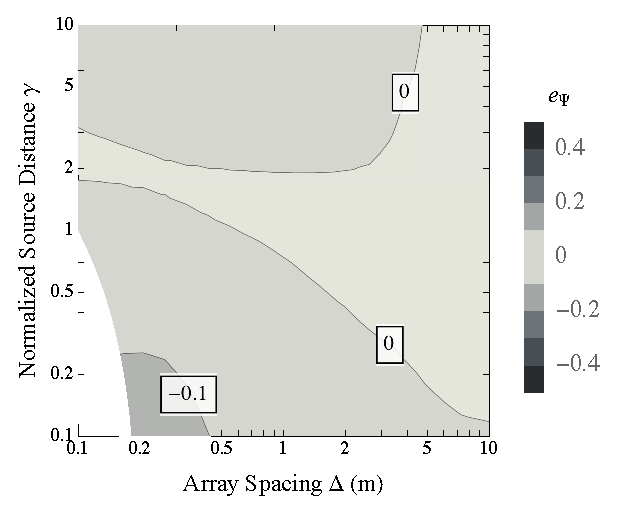
\includegraphics[width=\textwidth]{08_proposed_method/figures/merimaa2005_d_contour_validhybrid.eps}
		\caption{Proposed method}
		\label{fig:09_Thiergart_Comparison:Diffuseness_Errors:Hybrid}
	\end{subfigure}
	
	\caption[Contour plots of diffuseness errors for each interpolation method.]{
	Diffuseness errors $e_\Psi$ for microphone spacing $\Delta$ and normalized source distance $\gamma$.
  Contour lines are drawn in increments of $0.1$.
  \Figref{fig:09_Thiergart_Comparison:Diffuseness_Errors:Hybrid} has been reproduced from \figref{fig:08_Proposed_Method:Diffuseness_Errors:Hybrid}.}
	\label{fig:09_Thiergart_Comparison:Diffuseness_Errors}
\end{figure*}

This apparent deficiency in diffuseness of the time-frequency method suggests that the diffuse sound term in the sound field re-synthesis equation, \eqnref{eq:03_Navigation_Techniques:Thiergart_Synthesis}, is underestimated by the method.
Consequently, it may be relatively straightforward to modify the time-frequency method to correct for this behavior.
This is a topic for further development.

\section{Conclusions and practical implications}\label{sec:09_Thiergart_Comparison:Conclusions}
In this chapter, we presented numerical simulations conducted in order to characterize and compare the performance of the time-frequency interpolation method of \citet{Thiergart2013} to our proposed parametric interpolation method.
Following the simulation framework laid out in \chapref{chap:06_Simulation_Framework}, we simulated simple incident sound fields consisting of a two-microphone array and a single point-source, varying source distance and azimuth, as well as microphone spacing and listener position.
We first explored basic properties of the time-frequency method by computing the effective frequency responses induced by translation via the method across source azimuths.
Then, we conducted a more comprehensive analysis of the methods by computing, for a wide range of conditions, the metrics enumerated in \secref{sec:06_Simulation_Framework:Metrics} for sound level, spectral coloration, source localization, and diffuseness.
The analyses presented in this chapter yielded the following findings:
\begin{itemize}
\item the time-frequency method yields virtually exact sound levels for all conditions, and is particularly superior to the proposed method for interior sources;
\item the time-frequency method yields significantly larger spectral errors than the proposed method for microphone spacings larger than approximately $0.5$~m;
%\item that these larger errors will be perceptible as increased coloration is reinforced by established psychoacoustic results;
%\item while the precise origin of this coloration remains unclear, it may well be related to the presence of wider (but shallower) notches in the frequency responses induced by the time-frequency method compared to those induced by the proposed method;
\item the time-frequency method yields significantly smaller localization errors than the proposed method for interior sources with microphone spacings larger than approximately $1$~m; and
\item the time-frequency method does not sufficiently reproduce the diffuseness of a sound field, whereas the proposed method yields virtually exact diffuseness for almost all conditions.
\end{itemize}

%\subsection{Practical implications}
Taken together, the findings presented in this chapter suggest that the time-frequency method and the proposed method may each be more suitable in different practical domains.
For the present discussion, we define the following practically-relevant ``axes'':
\begin{enumerate}
\item the \textit{sparsity} of the microphone array, i.e., the size of the desired navigable region relative to the number of available microphones (e.g., $\sim\Delta/2$);
\item the \textit{intimacy} of the sound sources, i.e., the proximity of the sources to the navigable region (e.g., $\sim1/\gamma$); and
\item the \textit{complexity} of the sound field, i.e., the total number of sources and/or the reverberance of the recording environment.
\end{enumerate}
%These axes are illustrated in \figref{fig:09_Thiergart_Comparison:Practical_Axes}.
While the first two of these axes can be easily related to microphone spacing and normalized source distance, respectively, the third axis has not been directly explored here.
However, based on the construction of the time-frequency method, we speculate that this method may have difficulties accommodating multiple sources since, at each time-frequency bin, only a single point-source is created (see \secref{sec:03_Navigation_Techniques:Thiergart_Method}).
Consequently, the capability of this method to accurately reproduce multiple sources warrants further study.

%\begin{figure}[tb]
%	\includegraphics[width=\textwidth]{extras/figures/Practical_Axes_Diagram.pdf}
%	\caption{Illustration of the three practically-relevant axes defined in the text:
%	the sparsity of the microphone array,
%	the intimacy of the sound sources,
%	and the complexity of the sound field.
%	Empty circles indicate microphones,
%	filled circles indicate sources,
%	the filled rectangle indicates a scattering body,
%	and the hatched line indicates a reflective surface.}
%	\label{fig:09_Thiergart_Comparison:Practical_Axes}
%\end{figure}

Nevertheless, below, we identify several general principles with which to choose between the two methods in various applications spanning these axes:
\begin{enumerate}
% sparsity axis
\item[1a.] With a sparse microphone array (e.g., when covering a large room with only a few microphones), the time-frequency method will generally yield superior localization accuracy, whereas the proposed method will incur less spectral coloration.
\item[1b.] With a dense microphone array, the methods perform comparably to each other (i.e., neither method is particularly superior) in terms of localization accuracy and spectral coloration.
% intimacy axis
\item[2a.] When recording primarily intimate sources (e.g., an immersive recording of a small group of musicians), the time-frequency method will yield superior localization accuracy and will likely better convey source distance information (due to its accurate reproduction of sound level), whereas the proposed method will again incur less spectral coloration.
\item[2b.] When recording primarily distant sources (e.g., when covering the audience section only of a concert hall), the proposed method will yield smaller spectral and localization errors.
% complexity axis
\item[3a.] For an acoustically complex sound field (e.g., in a room with highly reflective surfaces and/or many scattering bodies), the proposed method is likely more suitable as it more accurately reproduces diffuseness and, potentially, the time-frequency method will fail to adequately reproduce many sources.
\item[3b.] For an acoustically simple sound field (e.g., an outdoor recording of a park with sparsely distributed sources), the time-frequency method will likely yield superior localization accuracy, and its deficiency in diffuseness will be less problematic.
\end{enumerate}

% Parameters:
% sparsity of microphone array: size of desired navigable region / number of microphones
% intimacy of sound field: presence of important sources with \gamma < 1
% sound field complexity: number of sources * reverberance of environment

% order of microphones
% movement of sources
% most important attributes: sound quality vs. spatial accuracy

While these principles specify the superior method for any given practical domain, another way of summarizing the results presented in this chapter is to determine the domains, in terms of these practical axes, over which each method yields \textit{accurate and superior} performance.
As we did not explore the complexity axis explicitly, here we omit that axis and focus only on the sparsity of the microphone array and the intimacy of the sources.
Additionally, since the level and diffuseness results are relatively straightforward (see \figreftwo{fig:09_Thiergart_Comparison:Level_Errors}{fig:09_Thiergart_Comparison:Diffuseness_Errors}, respectively), we omit those metrics as well.

Using the errors plotted in \figreftwo{fig:09_Thiergart_Comparison:Spectral_Errors}{fig:09_Thiergart_Comparison:Localization_Errors}, we first identify, for each method, regions of low coloration ($\rho_\eta < 3$~dB) and regions of accurate localization ($e_\nu < 10^\circ$).
We then determine the regions in which each method performs a) more accurately than that error limit and b) more accurately than, or at least comparably to, the other method.
These regions are sketched in \figref{fig:09_Thiergart_Comparison:Region_Plots}.

\begin{figure*}[t]
	\centering
	\begin{subfigure}[b]{0.49\textwidth}
		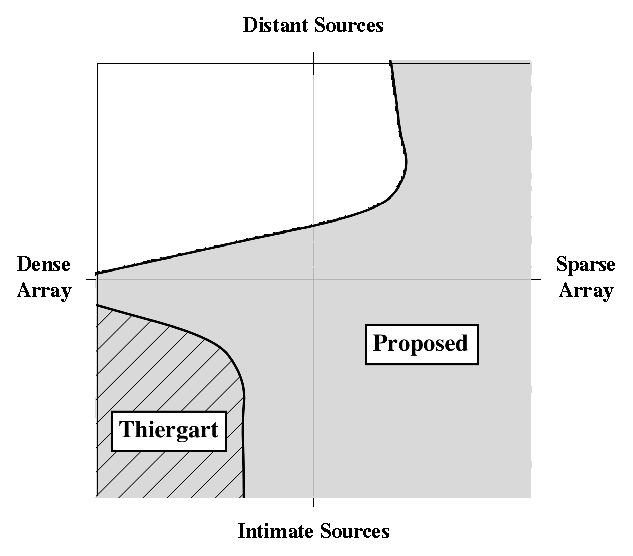
\includegraphics[width=\textwidth]{09_thiergart_comparison/figures/Coloration_Region_Plot}
		\caption{Coloration}
		\label{fig:09_Thiergart_Comparison:Region_Plots:Coloration}
	\end{subfigure}
	\hfill
	\begin{subfigure}[b]{0.49\textwidth}
		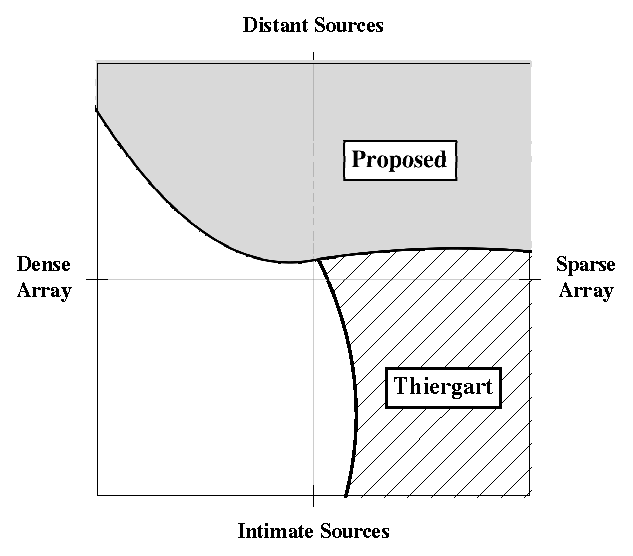
\includegraphics[width=\textwidth]{09_thiergart_comparison/figures/Localization_Region_Plot}
		\caption{Localization}
		\label{fig:09_Thiergart_Comparison:Region_Plots:Localization}
	\end{subfigure}
	
	\caption[Region plots of practical applicability of each interpolation method.]{
	Region plots illustrating accurate and superior methods in terms of spectral coloration (left panel) and localization accuracy (right) across practical applications with varying microphone array sparsity (horizontal axis) and sound source intimacy (vertical).
	The gray filled regions correspond to the proposed method and
	the hatched regions correspond to the time-frequency method of \citet{Thiergart2013}.
	Regions that are both filled and hatched indicate that the methods perform comparably;
	empty regions indicate that neither method satisfies the specified error limit.}
	\label{fig:09_Thiergart_Comparison:Region_Plots}
\end{figure*}

From these plots, we see that, in applications with distant sources and with a sparse microphone array, the proposed method yields accurate and superior performance in both coloration and localization.
Furthermore, for most applications with a sparse microphone array or with intimate sources, the proposed method yields accurate and often superior spectral coloration performance, and for most applications with distant sources, the proposed method yields accurate and superior localization performance.
The time-frequency method, however, yields accurate spectral coloration performance only for applications with a dense microphone array and with intimate sources, and the method yields accurate and superior localization performance only for applications with a sparse microphone array and with intimate sources.
Consequently, in such applications (with both a sparse microphone array and with intimate sources), the time-frequency method yields improved localization but degraded coloration performance compared to the proposed method.

% a more general discussion of practical things
A practical advantage of the time-frequency method is that it only requires first-order ambisonics microphones (which tend to be significantly less expensive than higher-order ones and require fewer recording channels, preamplifiers, etc.).
However, as shown in \secref{sec:08_Proposed_Method:Order_Dependence}, the performance of the proposed method does not vary significantly with order, so similar performance to that shown in this chapter would be achieved even with only $L_\text{in} = 1$.
Also, as mentioned in \secref{sec:09_Thiergart_Comparison:Simulations}, the time-frequency method fails to triangulate sources with azimuths of $|\varphi_0| = 90^\circ$.
While, in practice, a source azimuth of exactly $\pm 90^\circ$ is virtually impossible (e.g., due to positioning errors, noise, etc.), this does suggest that the triangulation calculation (see \eqnref{eq:03_Navigation_Techniques:Source_Triangulation}) may be very sensitive to small changes in azimuth near these extremes.
This issue might be easily avoided, however, by using $P > 2$ microphones arranged in a triangular or rectangular configuration, for example.

While the evaluation presented in this chapter has been purely numerical, we hope that the practical recommendations enumerated above will facilitate real-world implementations of these navigational methods.
Ideally, the conclusions drawn from these analyses will be borne out by future experimental investigations.
To that end, in the following chapter, we present an experimental validation of our numerical simulation framework (from \chapref{chap:06_Simulation_Framework} but which has been use throughout \chaprefthru{chap:07_Characterization_Extrapolation}{chap:09_Thiergart_Comparison}), which will serve to ground the findings presented throughout this thesis in experimentally measured data.

\section*{Acknowledgements}
This work was originally submitted by \citet{TylkaChoueiri2019d} to \textit{The Journal of the Audio Engineering Society}.